 \subsection{An User visualizes his History data through a customized research}
 
The User can access to its past data stored in the system, specifying the interval time of interest or the location in which the data were collected. If the User does not insert any preference, are shown all the available data, and the User can reads them performing a manual research.
The data can be visualized ordered by time or by location (e.g. the health data collected when the User were in the city of Milan).

\begin{table}[H]
	\centering
    
    \begin{tabular}{|p{3.5cm}|p{10.3cm}|}
    
    \hline
    
    \textbf{\large{Actors}}  			& \tabitem  User  				\\
    				 	
    \hline
    
    \textbf{\large{Goals}} 				&\ref{goal:user3}\\
    
     \hline
     
    \textbf{\large{Enter Condition}} & The User should be logged in.\\
    
    \hline
    \textbf{\large{Events Flow}}		& \begin{enumerate}[leftmargin=0.5cm]
                                          	\item The \emph{User}  presses the "History" button.
                                            \item The System asks to specify what kind of parameters he wants to see.
                                            \item The \emph{User} specifies the parameters of the data that wants to visualize.
                                            \item The \emph{User} can specify the time or the location range. 
                                            \item The System retrieves the informations requested from the database
                                            \item The System shows the data to the user.
                                            \item The \emph{User} selects the visualization order(time or location order).
                                            \item In case of localization data, the \emph{User} can view them more in detail on an interactive map pressing on the map button.            \end{enumerate}\\
                                            
    \hline
    
    \textbf{\large{Exit Condition}} 	& The User can examine the requested data. \\
    
    \hline
    
    \textbf{\large{Exception}} 			& \begin{enumerate}[leftmargin=0.5cm]                                           \item The requested data do not                                         exist in the database. 
                                        \end{enumerate}
                                        In this case the System shows an error message and invites the User to insert consistent preferences.\\
    
    \hline
    
    \end{tabular}
	
\end{table}
\begin{figure}[H]
    \centering
    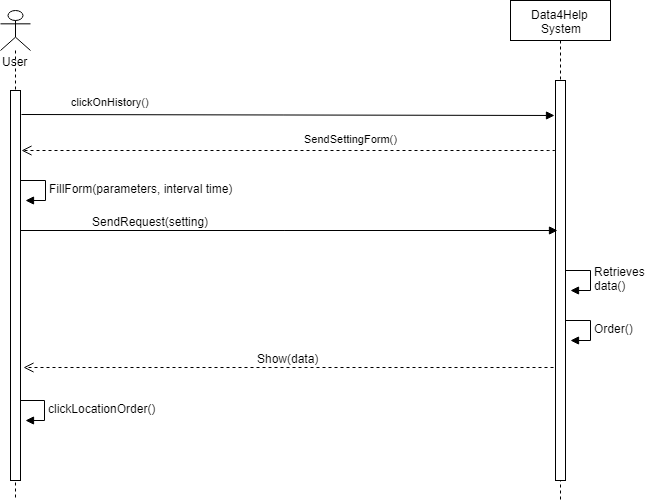
\includegraphics[scale=0.4]{rasdL/Pictures/history.png}
     \caption{In this use case the User performs a history search on his data specifying an interval time and visualizes them in location order}
    
\end{figure}
